\newpage
\section{Wymagania}

% Dla wymagań funkcjonalnych i niefunkcjonalnych
% Globalnie zakładam, że zagnieżdżone listy będą numerowane cyframi
\setenumerate{label*=\arabic*.}

W tej sekcji znajduje się lista wymagań jakie spełniać powinien budowany system.
Podane są one z podziałem na dwie kategorie. Pierwsza to wymagania funkcjonalne
określające funkcjonalności systemu oraz sposoby ich użycia. Druga natomist to
wymagania niefunkcjonalne, które opisują ilościowe i jakościowe warunki
działania systemu.

\subsection{Wymagania funkcjonalne}
\subsubsection{Klient}

Wymagania funkcjonalne dotyczące klientów zamawiających części w sklepie

\begin{enumerate}
  \item Dodanie nowego klienta
  \item Edycja danych klienta
  \begin{enumerate}
    \item Edycja adresu klienta
    \item Edycja adresu e-mail
  \end{enumerate}
  \item Edycja czułych danych klienta
  \begin{enumerate}
    \item Edycja hasła
    \item Edycja statusu (stały klient, nowy klient)
  \end{enumerate}
  \item Wyrejestrowanie się klienta
  \item Usunięcie klienta
\end{enumerate}

\subsubsection{Zamówienia}

Wymagania funkcjonalne dotyczące zamówień realizowanych przez sklep:

\begin{enumerate}
  \item Prezentacja zamówień
  \item Edycja, modyfikacja
  \begin{enumerate}
    \item Dodanie lub usunięcie produktu z zamówienia
    \item Zmiana ilości produktu
  \end{enumerate}
  \item Zmiana danych zamawiającego
  \item Usunięcie zamówienia w całości
  \item Edycja formy płatności
  \begin{enumerate}
    \item Płatność gotówką
    \begin{enumerate}
      \item Koszt w złotówkach
      \item Koszt w euro
      \item Koszt w wirtualnej walucie
    \end{enumerate}
    \item Płatność przelewem
    \item Płatność ratalna oparta o system szybkich pożyczek SuperBank
    \item Możliwość wpłaty zaliczki przed wysyłką
    \item Obniżenie kosztu o naliczone rabaty i zniżki
  \end{enumerate}
  \item Wybór sposobu potwierdzenia zamówienia (faktura, paragon)
  \item Generowanie faktury pro-forma dla danego zmówienia
  \item Zarządzanie terminem dostawy
  \item Ustawianie aktualnego stanu zamówienia.
\end{enumerate}
\subsubsection{Pracownik}

Wymagania funkcjonalne dotyczące obsługi pracowników w systemie:

\begin{enumerate}
  \item Zatrudnienie nowego pracownika
  \item Zwolnienie pracownika
  \item Ustalanie urlopów
  \begin{enumerate}
    \item Zgłaszanie próśb o urlop.
    \item Zarządzanie urlopami.
      \begin{enumerate}
        \item Rozpatrywanie próśb o urlop.
        \item Automatyczna aktualizacja statusów urlopów przez system.
      \end{enumerate}
  \end{enumerate}
\end{enumerate}


\pagebreak
\subsubsection{Opis przypadków użycia - klient}

Opis przypadków użycia wyjaśniające funkcjonalności związane z zarządzaniem
klientami:

\begin{enumerate}
  \item Rejestracja klienta \\
  \begin{tabularx}{\linewidth}{ c X }
  Aktor: & Klient \\
  Opis: & Możliwość rejestracji nowego klienta.\\
  \end{tabularx}
   \begin{enumerate}
    \item Klient uruchamia stronę internetową sklepu i wybiera opcję rejestracji
    \item Klient wstawia swoje dane osobowe i wybiera domyślny model płatności
    (kartą, za pobraniem itp.)
    \item System sprawdza wstawione dane (takie same hasła, czy istnieje już
    zarejestrowany w systemie użytkownik, czy istnieje podany adres e-mail itp.)
    \item System wysyła e-mail powitalny na adres podany przez klienta
    \item W ciągu określonego, zdefiniowanego czasu klient wybiera przesłany w
    e-mailu link, stając się pełnoprawnym użytkownikiem sklepu
  \end{enumerate}
  \item Złożenie zamówienia \\
  \begin{tabularx}{\linewidth}{ c X }
  Aktor: & Klient \\
  Opis: & Przedstawienie sposobu złożenia zamówienia.\\
  \end{tabularx}
  \begin{enumerate}
    \item Klient uruchamia stronę internetową sklepu i wyszukuje interesujące go
    produkty
    \item W momencie znalezienia pasującego produktu użytkownik wybiera opcję
    dodania do koszyka
    \item Po zakończeniu wyszukiwania użytkownik wybiera opcję przejścia do kasy
    \item System sprawdza, czy użytkownik jest zalogowany. Jeśli nie, procesuje
    przypadek użycia Logowanie do Systemu
    \item System sprawdza, czy użytkownik jest stałym klientem. Jeśli tak,
    dolicza rabat do ustalonej ceny (do sumy cen poszczególnych produktów)
    \item Użytkownik wybiera sposób płatności
    \item System dodaje do wcześniej ustalonej ceny koszty wynikające ze sposobu
    płatności
    \item Użytkownik wybiera sposób dostawy (poczta, kurier, odbiór osobisty
    itp.)
    \item System dodaje do ceny koszty wynikające ze sposobu dostawy
    \item Użytkownik, po sprawdzeniu wszystkich danych, decyduje się na złożenie
    zamówienia - po tym momencie nie może już ono być cofnięte
    \item System wysyła do użytkownika e-mail potwierdzający wraz z przewidywaną
    datą realizacji zamówienia
  \end{enumerate} 
  \item Edycja danych klienta \\
  \begin{tabularx}{\linewidth}{ c X }
  Aktor: & Klient \\
  Opis: & Możliwość zmiany, uzupełnienia danych osobowych klienta.\\
  \end{tabularx}
  \begin{enumerate}
    \item Klient uruchamia witrynę internetową sklepu
    \item Klient loguje się do systemu (tylko osoba zalogowana może zmieniać
    swoje dane)
    \item Klient edytuje wybrane pozycje ze swojego opisu (adres, numer
    telefonu itp.)
    \item W przypadku zmiany hasła klient proszony jest o podanie starego jak i
    nowego (dwukrotnie) hasła
    \item Klient zatwierdza wprowadzone zmiany
    \item System wysyła na podany przez użytkownika adres e-mail (nowy, jeśli
    to adres e-mail był jedną ze zmienianych wartości) informację o zmianie.
  \end{enumerate}
  \item Wyrejestrowanie się klienta \\
  \begin{tabularx}{\linewidth}{ c X }
  Aktor: & Klient \\
  Opis: & Klient ma możliwość w każdym momencie usunąć swoje konto z systemu.\\
  \end{tabularx}
  \begin{enumerate}
    \item Klient uruchamia witrynę internetową i loguje się na swoje konto
    (przypadek użycia Logowanie Do Systemu)
    \item Klient wybiera opcję usunięcia danych
    \item System sprawdza, czy istnieją niezrealizowane (oczekujące) zamówienia.
    Jeśli tak, wyświetla się alert z informacją, czy dane zamówienie zostało już
    wcześniej opłacone
    \item Jeśli istniały już zamówienia, które zostały opłacone a nie zostały
    jeszcze zrealizowane, system zleca odesłanie określonej kwoty pieniężnej z
    powrotem na konto użytkownika (z pominięciem kosztów obsługi)
    \item Klient zostaje poproszony o podanie przyczyn swojej decyzji -
    wypełnianie jest nieobowiązkowe
    \item Dane przechowywane są przez Okres Przechowywania Danych (wymaganie
    prawne - patrz Wymagania niefunkcjonalne punkt \ref{itm:OPD}). W tym
    czasie klient może ponownie zarejestrować się w systemie bez utraty poprzednich danych
    \item W przypadku braku ponownej rejestracji dane zostają na stałe usunięte
    z firmowej bazy danych
  \end{enumerate}
  \item Usunięcie klienta \\
  \begin{tabularx}{\linewidth}{ c X }
  Aktor: & Pracownik \\
  Opis: & Klienta można usunąć administracyjnie na przykład z powodów
  naruszenia regulaminu.\\
  \end{tabularx}
  \begin{enumerate}
    \item Pracownik sklepu wyszukuje klienta o konkretnym imieniu i nazwisku
    (lub według innych kryteriów)
    \item Pracownik wybiera opcję usunięcia klienta. 
    \item Pracownik wpisuje powód, dla którego usuwa użytkownika (informacja ta
    będzie przesłana do klienta w wiadomości e-mail)
    \item Pracownik wypełnia dane dotyczące kwestii niezrealizowanych zamówień i
    nieotrzymanych płatności
    \item Obie informacji (z poprzednich 2 kroków) są przekazywane na podany
    przez użytkownika adres e-mail
    \item Dane są przechowywane przez Okres Magazynowania Danych (patrz
    Wymagania Niefunkcjonalne punkt \ref{itm:OMD}) - w tym czasie użytkownik
    może złożyć reklamację i ewentualnie odzyskać dostęp do konta
    \item Po tym czasie, jeśli prośba o przywrócenie konta nie zostanie
    pozytywnie rozpatrzona, dane są na stałe usuwane z systemu
  \end{enumerate}
\end{enumerate}
\subsubsection{Opis przypadków użycia - zamowienia}

Przypadki użycia wyjaśniające funkcjonalności systemu związane z zarządzaniem
zamówieniami.

\begin{enumerate}
  \item Prezentacja zamówień\\
  \begin{tabularx}{\linewidth}{ c X }
  Aktor: & Pracownik \\
  Opis: & Prezentacja panelu z listą wszystkich zamówień znajdujących się w
  systemie oraz możliwościami kontroli i zarządzania nimi.\\
  \end{tabularx}
	\begin{enumerate}
	  \item Pracownik loguje się w Panelu Zarządzania
	  \item Wybiera Panel Zarządzania Zamówieniami
	  \item Wyświetlana jest lista zamówień z możliwością modyfikacji widoków
	  oraz panelem opcji (wszystkie opisane w poniższych przypadkach użycia)
	\end{enumerate}

  \item Edycja, modyfikacja zamówień\\
  \begin{tabularx}{\linewidth}{c X}
  Aktor: & Pracownik \\
  Opis: & Funkcjonalność umożliwia modyfikację produktów w zamówieniu oraz
  zmianę danych odbiorcy.
  \end{tabularx}
	\begin{enumerate}
	  \item Pracownik po autoryzacji w panelu sterowania systemu, przechodzi do
	  panelu Zarządzania Zamówieniami (patrz Zamowienia przypadek użycia 1)
	  \item Z wyświetlonej przez system listy zamówień, pracownik wybiera jeden
	  element
	  \item W celu edycji produktów:
		\begin{enumerate}
		  \item Wybiera opcję podglądu zawartości zamówienia
		  \item Z wyświetlonej listy zamówionych produktów zaznacza jedną pozycję
		  \item Wybiera opcję edycji
		  \item Otrzymuje informacje o konkretnym produkcie (jego ID, szczegółowy opis)
		  oraz zamówioną ilość oraz podsumowanie (cenę, informację o udzielonych rabatach na dany produkt)
		  \item Pole z ilością produktu umożliwia modyfikację – wystarczy wprowadzić
		  liczbę z zakresu od 1 do maksymalnej liczby aktualnie dostępnych produktów w
		  magazynie (0 nie wchodzi w zakres bo do tego służy funkcja usunięcia)
		\end{enumerate}
	  \item W celu usunięcia produktu:
		\begin{enumerate}
		  \item Wybiera opcję podglądu zawartości zamówienia
		  \item Z wyświetlonej listy zamówionych produktów zaznacza jedną pozycję
		  \item Wybiera opcję Usuń
		  \item System pyta o potwierdzenie i po akceptacji dokonuje wykluczenia
		  produktu z zamówienia oraz wysyła powiadomienie do Zamawiającego
		\end{enumerate}
	  \item W celu dodania produktu:
		\begin{enumerate}
		  \item Wybiera opcję podglądu zawartości zamówienia
		  \item Wybiera opcję Dodaj produkt
		  \item Otworzony zostaje system zakupowy\\ 
		  (przebieg wyboru produktu - opisany w przypadkach użycia odnoszących się do
		  Produktów)
		  \item Po wybraniu produktu system wyświetla informację o tym jakie zostaną
		  wprowadzone zmiany i czeka na akceptację
		  \item Po akceptacji, zamówienie zostaje zmodyfikowane (produkt dodany),
		  koszt zaktualizowany oraz system informuje odbiorcę zamówienia (klienta) o
		  zaszłych zmianach – za pomocą wiadomości email (z ewentualną poprawioną
		  fakturą pro-forma, jeśli była zaznaczona taka opcja) 
	  \end{enumerate} %koniec alternatywy Dodania produktu
	\end{enumerate} %koniec UC Edycja, modyfikacja zamówień
  
  \item Zmiana danych zamawiającego\\
  \begin{tabularx}{\linewidth}{c X}
  Aktor: & Pracownik \\
  Opis: & Można zmienić dane odbiorcy na potrzeby danego zamówienia (zmiana
  danych tylko w ramach konkretnej faktury). Dotyczy to w szczególności adresu i
  danych osobowych osoby odpowiedzialnej za zamówienie.
  \end{tabularx}  
	\begin{enumerate}
	  \item Pracownik po autoryzacji w panelu sterowania systemu, przechodzi do
	  panelu Zarządzania Zamówieniami (patrz Zamówienia przypadek użycia 1)
	  \item Z wyświetlonej przez system listy zamówień, pracownik wybiera jeden
	  element i wybiera opcję Zmień Dane Odbiorcy
	  \item System prezentuje aktualnie dane odbiorcy (mogą to być aktualne dane
	  klienta, albo już wcześniej modyfikowane dane osobowe wprowadzone specjalnie w
	  ramach tego zamówienia)
	  \item Pracownik modyfikuje wybraną przez siebie składową danych (wszystkie
	  elementy pozwalają na edycję) i zatwierdza wprowadzone zmiany
	  \item System wyświetla zapytanie o potwierdzenie zmian i po jego akceptacji
	  wysyła powiadomienie do klienta o zaszłych zmianach – wiadomość drogą
	  elektroniczną
	\end{enumerate}

  \item Usunięcie zamówienia w całości\\
  \begin{tabularx}{\linewidth}{c X}
  Aktor: & Pracownik \\
  Opis: & Istnieje możliwość anulowania zamówienia – na życzenie klienta lub z
  powodów biznesowych sklepu.
  \end{tabularx}  
	\begin{enumerate}
	  \item Pracownik po autoryzacji w panelu sterowania systemu, przechodzi do
	  panelu Zarządzania Zamówieniami (patrz Zamówienia przypadek użycia 1)
	  \item Z wyświetlonej przez system listy zamówień, pracownik wybiera jeden
	  element i wybiera opcję Usuń zamówienie
	  \item System wyświetla ostrzeżenie (wraz ze szczegółową informacją o
	  zamówieniu) i pyta o potwierdzenie
	  \item Pracownik potwierdza chęć usunięcia danego zamówienia. Ma też możliwość
	  wpisania krótkiego uzasadnienia tej operacji
	  \item System dokonuje usunięcia oraz wysyła powiadomienie o anulowaniu
	  zamówienia do zamawiającego (drogą elektroniczną)
	\end{enumerate}

  \item Edycja formy płatności\\
  \begin{tabularx}{\linewidth}{c X}
  Aktor: & Pracownik \\
  Opis: & Pracownik ma możliwość zmiany początkowo wybranej formy płatności
  danego zamówienia. Odbywa się to na wniosek zamawiającego lub osoby
  odpowiedzialnej za zamówienia po stronie Sklepu.
  \end{tabularx}    
	\begin{enumerate}
	  \item Z listy zamówień pracownik wybiera jedno i wybiera opcję Zmiana formy
	  płatności
	  \item System prezentuje widok wyboru pomiędzy dostępnymi formami płatności
	  (specyfikacja w wymaganiach niefunkcjonalnych)
	  \item Pracownik dokonuje wyboru formy oraz waluty.
	  \item System powiadamia klienta o zmianie formy płatności drogą elektroniczną.
	\end{enumerate}

  \item Wybór sposobu potwierdzenia zamówienia\\
  \begin{tabularx}{\linewidth}{c X}
  Aktor: & Pracownik \\
  Opis: & Możliwość zmiany sposobu udokumentowania przeprowadzonej transakcji
  (zazwyczaj będzie to faktura albo paragon). Powodem takich zmian mogą być
  nawet regulacje prawne.
  \end{tabularx}	
	\begin{enumerate}
	  \item Z listy zamówień pracownik wybiera jedno i wybiera opcję Zmiana
	  Potwierdzenia Transakcji
	  \item System prezentuje widok wyboru pomiędzy dostępnymi sposobami
	  potwierdzenia (udokumentowania) prowadzonej transakcji.
	  \item Pracownik dokonuje wyboru oraz może uruchomić proces generacji
	  dokumentu.
	  \item W przypadku generacji dokumenty system wyświetla go pracownikowi.
	  \item Po akceptacji informacje o zmianie wraz z dokumentami wysyłane są drogą
	  elektroniczną do klienta.
	\end{enumerate}

  \item Generowanie faktury pro-forma dla danego zmówienia\\
  \begin{tabularx}{\linewidth}{c X}
  Aktor: & Pracownik \\
  Opis: & Możliwość utworzenie faktury pro-forma na podstawie danego zamówienia
  oraz przesłanie jej klientowi drogą elektroniczną lub wydruk.
  \end{tabularx}
	\begin{enumerate}
	  \item Z listy zamówień pracownik wybiera jedno i wybiera opcję Generuj
	  Pro-Forma
	  \item Dla wybranego zamówienia system generuje pełną fakturę po czym
	  prezentuje ją pracownikowi
	  \item Pracownik ma możliwość odrzucenia lub akceptacji dokumentu.
	  \item W przypadku akceptacji system wyświetla widok wyboru z opcjami wysyłki
	  do klienta.
	  \item Po wybraniu pożądanej opcji przez pracownika, system wysyła dokument do
	  klienta albo do drukarki.
	\end{enumerate}

  \item Zarządzanie terminem dostawy\\
  \begin{tabularx}{\linewidth}{c X}
  Aktor: & Pracownik \\
  Opis: & Termin realizacji zamówienia może być modyfikowany dowolnie w
  zależności od możliwości biznesowych Sklepu.
  \end{tabularx}
	\begin{enumerate}
	  \item Z listy zamówień pracownik wybiera jedno i wybiera opcję Edycji Daty
	  Realizacji
	  \item System prezentuje widok kalendarza z zaznaczoną dotychczasową datą
	  realizacji.
	  \item Pracownik przesuwa datę realizacji projektu i ma możliwość podania
	  wiadomości wyjaśniającej modyfikację.
	  \item System wysyła powiadomienie o zmianie terminu do klienta wraz z
	  informacją wyjaśniającą wpisaną przez pracownika.
	\end{enumerate}

  \item Ustawianie aktualnego stanu zamówienia\\
  \begin{tabularx}{\linewidth}{c X}
  Aktor: & Pracownik \\
  Opis: & Zamówienie może znajdować się w pewnych stanach realizacji (np. w
  przygotowaniu, w realizacji, wysłane - konkretne stany określają wymagania
  niefunkcjonalne). Istnieje możliwość zmiany aktualnego stanu zamówienia.
  \end{tabularx}
	\begin{enumerate}
	  \item Z listy zamówień pracownik wybiera jedno i wybiera opcję Zmień Stan
	  \item System prezentuje widok z dostępnymi stanami dla danego zamówienia
	  \item Pracownik dokonuje wyboru i zatwierdza zmiany.
	  \item Jeśli pracownik wybiera opcję Powiadom, to system powiadamia klienta o
	  zmianie stanu jaka nastąpiła i przesyła krótkie wyjaśnienie.
	\end{enumerate}
	 
\end{enumerate}

\subsubsection{Opis przypadków użycia - pracownik}

Opis przypadków użycia dotyczących funkcjonalności związanych z zarządzaniem
pracownikami:

\begin{figure}[h!]
    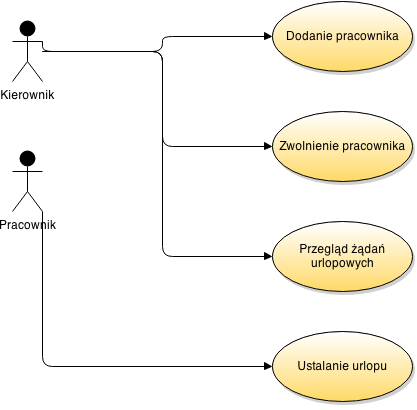
\includegraphics[width=\textwidth,
    height=0.5\textheight]{graphics/UseCase/Pracownik/UseCaseDiagram.png}
  \caption{Diagram przypadków użycia związanych z procesowaniem danych
  pracowników}
\end{figure}

\begin{enumerate}
	
	  \item Dodawanie pracownika \\
  
  Opis słowny - ten przypadek użycia wspiera proces rozwoju firmy poprzez
  zatrudnianie nowych pracowników. Dane na temat wszystkich osób związanych ze
  sklepem są lepiej wykorzystywane jeśli są zarządzane przez system
  informatyczny. Aby uruchomić tą procedurę należy mieć specjalne uprawnienia
  jakie posiadają wyznaczeni pracownicy, czyli Kierownicy.
  
  \begin{longtable}{|p{5cm}|p{7cm}|}
 	\hline
	\textbf{Aktor} & Kierownik \\
	\hline
	\textbf{Warunki początkowe} & Kierownik zalogowany, posiadający wszelkie dane
	nowego pracownika\\
	\hline
	\textbf{Opis przebiegu interakcji} & Wybór panelu zarządzania sklepem,
	wypełnienie danych pracownika i potwierdzenie zapisu \\
	\hline
	\textbf{Sytuacje wyjątkowe} & Błędne dane, dany pracownik już zarejestrowany \\
	\hline
	\textbf{Warunki końcowe} & Zarejestrowanie nowego pracownika w systemie \\
	\hline
 \end{longtable}
  
  \begin{tabularx}{\linewidth}{ c X }
  Aktor: & Kierownik \\
  \end{tabularx}
   \begin{enumerate}
    \item Kierownik uruchamia stronę internetową panelu zarządzania sklepem
    i~wybiera opcję rejestracji.
    \item Kierownik wprowadza dane osobowe zatrudnianego pracownika.
    \item System sprawdza wstawione dane (czy istnieje już zarejestrowany
    w~systemie użytkownik, czy istnieje podany adres e-mail itp.)
    \item System wysyła na adres e-mail pracownika podany przez~kierownika
    wiadomość powitalną wraz z~linkiem umożliwiającym aktywowanie konta oraz
    ustalenie hasła.
    \item W ciągu określonego, zdefiniowanego czasu pracownik odwiedza stronę
    o~adresie przesłanym w~wiadomości powitalnej i ustala hasło dla konta.
  \end{enumerate}

	Dodawanie pracownika - scenariusz alternatywny - błąd danych
	\begin{enumerate}
	  \item Kroki 1-3 scenariusza głównego
	  \item System wyświetla komunikat informujący o miejscu oraz typie błędu w
	  wprowadzonych danych
	  \item Dane zostają poprawione
	  \item Kroki następne scenariusza głównego od 3 włącznie.
	\end{enumerate}
	
	Dodawanie pracownika - scenariusz alternatywny - pracownik już zarejestrowany
	\begin{enumerate}
	  \item Kroki 1-3 scenariusza głównego
	  \item System oświadcza, że wprowadzone dane odpowiadają istniejącemu już
	  pracownikowi - wskazując pokrywające się informacje
	  \item Po akceptacji, formularz jest odrzucany.
	\end{enumerate}

	  \item Zwolnienie pracownika \\
  
  Opis słowny - współpraca z pracownikiem kiedyś dobiega końca, w takiej
  sytuacji uprawniona osoba musi usunąć takiego pracownika z systemu poprzez
  opcję zwolnienia. Informacje o tej osobie nie są usuwane bezpowrotnie lecz
  archiwizowane zgodnie z przepisami aktualnego prawa.
  
  \begin{longtable}{|p{5cm}|p{7cm}|}
 	\hline
	\textbf{Aktor} & Kierownik \\
	\hline
	\textbf{Warunki początkowe} & Kierwonik zalogowany	\\
	\hline
	\textbf{Opis przebiegu interakcji} & Wyświetlenie listy pracowników,
	zaznaczenia konkretnej osoby, wybór opcji zwolnienia \\
	\hline
	\textbf{Sytuacje wyjątkowe} & Brak \\
	\hline
	\textbf{Warunki końcowe} & Wybrany pracownik nie pojawia się więcej na liście
	pracowników, jego dane są zarchiwizowane. 	\\
	\hline
 \end{longtable}
  
  \begin{tabularx}{\linewidth}{ c X }
  Aktor: & Kierownik \\
  \end{tabularx}
   \begin{enumerate}
    \item Kierownik uruchamia stronę internetową panelu zarządzania sklepem i~wybiera panel zarządzania pracownikami.
    \item Kierownik wyszukuje odpowiedniego pracownika.
    \item System wyświetla pracowników spełniających zadane kryteria wyszukiwania.
    \item Kierownik wybiera odpowiedniego pracownika.
    \item Kierownik wybiera opcję ,,Zwolnij''.
    \item System wyświetla formularz zwolnienia.
    \item Kierownik wypełnia formualrz podając przyczynę zwolnienia oraz datę od której pracownik ma być zwolniony.
    \item System sprawdza poprawność formualrza (np. czy można zwolnić pracownika w terminie wskazanym przez kierownika).
    \item W przypadku błędów system wyświetla odpowiedni komunikat, a kierownik poprawia dane w formularzu.
    \item System wyświetla prośbę o potwierdzenie operacji (dane pracownika oraz pytanie czy na pewno intencją kierownika
    było jego zwolnienie).
    \item Pracownik zatwierdza operację.
    \item System zapisuje informację o zwolnieniu pracownika.
    \item W momencie zaczęcia obowiązywania zwolnienia, system archiwizuje dane pracownika i~usuwa
    go~z~grupy zatrudnionych osób.
  \end{enumerate}

  \begin{figure}[H]
    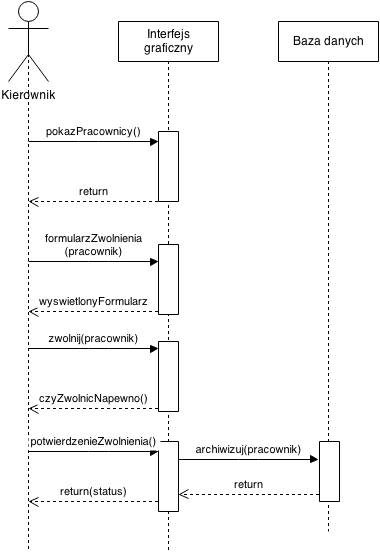
\includegraphics[width=\textwidth,
    height=0.5\textheight]{graphics/UseCase/Pracownik/ZwolnieniePracownika.png}
  \caption{Diagram sekwencji dla przypadku użycia Zwolnienie pracownika -
  scenariusz główny}
\end{figure}  
	\item Ustalanie urlopu \\

	Opis słowny - w nowoczesnych firmach przyjaznych pracownikowi kwestia urlopu
	jest niezwykle ważna. Po pierwsze konieczne jest zapewnienie firmie rąk do
	pracy. Po drugie zadowolony pracownik jest najcennieszy, dlatego istotny jest
	kompromis pomiędzy dniami urlopowymi, a pracującymi (globalnie, dla
	wszystkich). Ta funkcja systemu umożliwia zgłaszanie chęci wykorzystania czasu
	urlopu - wyrażenie swoich preferencji urlopowych przez pracownika

  \begin{longtable}{|p{5cm}|p{7cm}|}
 	\hline
	\textbf{Aktor} & Pracownik \\
	\hline
	\textbf{Warunki początkowe} & Pracownik zalogowany, posiada niewykorzystane
	dni urlopowe\\
	\hline
	\textbf{Opis przebiegu interakcji} & Wybór panelu urlopów,
	zaznaczenie preferowanych terminów, oczekiwanie na akceptację \\
	\hline
	\textbf{Sytuacje wyjątkowe} & Niezgodność liczby dni urlopu w stosunku do
	zaznaczonego okresu preferowanego urlopu - wymagana korekta
	\\
	\hline
	\textbf{Warunki końcowe} & Wysłanie preferencji urlopowych do akceptacji przez
	kierownika
	\\
	\hline
 \end{longtable}
  

  \begin{tabularx}{\linewidth}{ c X }
  Aktor: & Pracownik \\
  \end{tabularx}
  \begin{enumerate}
    \item Pracownik uruchamia aplikację internetową sklepu i loguje się do systemu.
    \item Pracownik wybiera panel urlopów.
    \item System informuje pracownika o ilości dni urlopowych pozostałych do wykorzystania.
    \item Pracownik dodaje do kalendarza firmowego nowe żądanie urlopu.
    \item Pracownik uzupełnia dane dotyczące czasu przebywania na urlopie (datę początkową oraz datę końcową).
    \item System sprawdza, czy żądanie pracownika jest poprawne (np. czy pracownik może wziąć tak długi urlop).
    Jeśli nie, pracownik jest informowany o przyczynie błędu i musi ponownie wypełnić dane o urlopie.
    \item System zapisuje żądanie urlopu i informuje użytkownika o zmianie statusu żądania
    na~,,Oczekiwanie na odpowiedź kierownika''.
    \item Kierownik przegląda żądanie zgodnie ze scenariuszem ,,Przeglądanie żądań urlopowych''.
    \item Pracownik jest informowany o rozpatrzeniu żądania.
  \end{enumerate} 
  

	  \item Przeglądanie żądań urlopowych \\
  
  Opis słowny - preferencje odnośnie terminu wykorzystania zasłużonego urlopu
  przez pracowników spływają do Kierownika i wymagają jego akceptacji. Ten
  przypadek użycia nakreśla procedurę jaką należy wykonać w tym celu.
  
  \begin{tabularx}{\linewidth}{ c X }
  Aktor: & Kierownik \\
  Opis: & Możliwość przeglądania i rozpatrywania żądań urlopowych napływających od pracowników.\\
  \end{tabularx}
  \begin{enumerate}
    \item Kierownik loguje się do aplikacji internetowej systemu.
    \item Kierownik wybiera panel zarządzania pracownikami i przechodzi do sekcji ,,Urlopy''.
    \item System wyświetla kalendarz, w którym umieszczone są terminy urlopów.
    \item Kierownik ustawia odpowiednie filtry urlopów (np. wyświetlanie tylko nierozpatrzonych żądań).
    \item Kierownik wybiera jeden z urlopów i zmienia jego status.
    \item System sprawdza czy zmiana statusu jest poprawna (np. czy nie wystąpiła zmiana statusu z ,,Zrealizowany'' na ,,Odwołany'').
    \item W przypadku błędnej operacji system informuje o tym kierownika.
  \end{enumerate}
	
\end{enumerate}
\newpage
\subsection{Wymagania niefunkcjonalne}

\begin{enumerate}
  \item Pojemność: \\ 
  System powinien mieć możliwość przechowywania danych o 100 tys.
  użytkowników 
  \item Wydajność: \\ 
  System powinien obsługiwać bez znaczącego spadku wydajności 400
  użytkowników ``jednocześnie''. Zakładając, że użytkownik będzie wymagał
  maksymalnie 20 odświeżeń widoku systemu na minutę (jedna podstrona na 3
  sekundy). System powinien działać z wydajnością 8000 odświeżeń/minutę. 
  \item System powinien być dostępny dla klientów 24 godziny na dobę 7 dni w
  tygodniu (możliwe są przerwy konserwacyjne, jednak nie dłuższe niż 4 godziny na miesiąc pracy) 
  \item Średni czas naprawy (MTTR - ang. Mean Time to Recover) na poziomie
  1~godziny
  \item System powinien umożliwiać klientom dostęp z dowolnego miejsca na
  świecie za pomocą sieci Internet oraz jego działanie powinno być niezależne od
  używanej platformy systemowo-sprzętowej użytkownika.
  \item Dane osobowe muszą być przetwarzane zgodnie z ustawą o ochronie danych
  osobowych z dnia 29 sierpnia 1997 r. 
  \item Klient powinien mieć dostęp do wszystkich swoich danych (łącznie z
  możliwością ich aktualizacji i usunięcia) zgodnie z polskim prawem
  \item Dane te powinny być chronione w zależności od ich poziomu poufności
  (dane do autoryzacji powinny być zabezpieczone przed możliwością odczytu nawet
  przez administratora) 
  \item Komunikacja pomiędzy klientem (przeglądarką internetową, aplikacją
  mobilną itp.) powinna być szyfrowana w sposób uniemożliwiający odczytanie czułych informacji
  \item System powinien mieć wbudowane procedury przeciwdziałania sytuacjom
  awaryjnym - procedury uruchamiane przez administratora
  \begin{enumerate}
    \item Procedury sprawdzenia spójności danych - po odzyskaniu sprawności, np.
    po awarii sprzętu
    \item Procedury uruchamiane w przypadku wykrycia włamania (między innymi,
    odłączenie systemu od sieci Internet, zablokowanie modyfikacji elementów
    systemu itp.)
  \end{enumerate} 
  \item System posiadać będzie hierarchię uprawnień (ról) dla użytkowników,
  przydzielanych im w celu umożliwienia korzystania z dodatkowych
  funkcjonalności
  \item System domyślnie powinien nadawać użytkownikowi uprawnienia nie większe
  niż niezbędne mu do poprawnego zamawiania produktów i zarządzania swoim
  kontem
  \item System powinien umożliwiać automatyczne wysyłanie klientowi wiadomości
  e-mail (z prośbą o potwierdzenie zmiany hasła czy akceptacji warunków rejestracji)
  \item System powinien umożliwiać użytkownikowi zmianę (w ograniczonym stopniu)
  już złożonego zamówienia (zmiana adresu przed wysyłką itp.) bez konieczności
  ingerencji pracownika sklepu
  \item System powinien być zdolny do wyświetlania informacji w wielu językach.
  Początkowo będzie to język polski i angielski. Istnieje jednak możliwość
  rozszerzenia o kolejne.
  \item \label{itm:OPD} Okres Przechowywania Danych - to czas przez który będą
  przechowywane dane użytkownika sprzed ich zmiany lub wyrejestrowania - system zapewnia
  magazynowanie tych danych co najmniej przez 7 dni.
  \item \label{itm:OMD} Okres Magazynowania Danych to czas 30 dni przez które
  system powinien przechowywać dane o klientach po usunięciu konta klienta (czas ten może się
  zmienić z powodów prawnych)
  \item \label{itm:Platnosci} System wspiera następujące formy płatności:
  \begin{enumerate}
    \item Płatność gotówką
    \item Przelew bankowy
    \item Płatność ratalna w oparciu o zewnętrzną usługę bankową
  \end{enumerate}
  Waluty: polski złoty, euro, bitcoin
  \item \label{itm:PotwierdzenieTransakcji} Forma potwierdzenia transakcji:
  faktura albo paragon
  \\
  System powinien umożliwiać generowanie tych dokumentów oraz ich wydruk.
  
\end{enumerate}
